\wde{Buffer Overflow}{
    Buffer overflows arise when a region of memory exceeds its allocated size, resulting in the overwriting of adjacent memory that may be used elsewhere in the program. This can lead to unexpected behavior in the program's execution.
    A buffer overflow exploits the stack layout to typically overwrite the return address of a function to 
    perform arbitrary code execution (shellcode or return-to-libc).
    This attacks the integrity of the program and can lead to privilege escalation.
    It's also possible to attack the availability of the program by causing a denial of service - by crashing the program.
}

\wde{Out-by-one/Arithmetic Errors}{
    Can lead to buffer overflows, memory corruption, and other security vulnerabilities.
}

\wde{Faulty/Missing Error Condition Checking}{
    Not checking for error conditions can lead to unexpected behavior and security vulnerabilities.
}

\wde{Format String Vulnerabilities}{
    Can lead to memory corruption, arbitrary code execution, and other security vulnerabilities.
    In C and C++, the \texttt{printf} function is vulnerable to format string attacks if the format string is user-controlled.
}
\wde{Stack Layout}{
    \begin{center}
        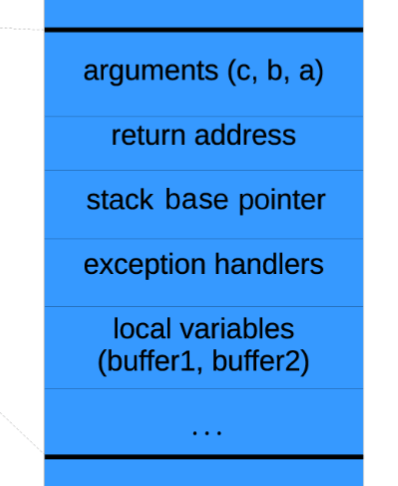
\includegraphics[width=0.5\linewidth]{images/stack-layout.png}
    \end{center}
The above diagram shows the layout of the stack in memory. The stack grows downwards, with the stack pointer pointing to the top of the stack. The stack frame contains the return address, arguments, local variables, and saved registers. The frame pointer points to the base of the current stack frame (current function).
}